\documentclass[aspectratio=169]{beamer}

\usetheme{Madrid}
\usecolortheme{rose}
\usefonttheme{professionalfonts}

\usepackage[T1]{fontenc}
\usepackage[utf8]{inputenc}
\usepackage{amsmath,amssymb,mathtools}
\usepackage{booktabs}
\usepackage{array}
\usepackage{hyperref}
\usepackage{tikz}
\usetikzlibrary{arrows.meta,positioning,shapes.geometric,fit,calc}

\hypersetup{
  colorlinks=true,
  linkcolor=magenta!70!black,
  urlcolor=magenta!70!black,
  citecolor=magenta!70!black
}

\definecolor{softpink}{HTML}{F7DCE5}
\definecolor{softpinkdark}{HTML}{B85C7B}
\definecolor{softpinkaccent}{HTML}{E89AB4}

\setbeamercolor{structure}{fg=softpinkdark}
\setbeamercolor{frametitle}{fg=white,bg=softpinkdark}
\setbeamercolor{title}{fg=white,bg=softpinkdark}
\setbeamercolor{subtitle}{fg=white,bg=softpinkdark}
\setbeamercolor{author}{fg=white,bg=softpinkdark}
\setbeamercolor{block title}{bg=softpinkdark!85,fg=white}
\setbeamercolor{block body}{bg=softpink!35,fg=black}
\setbeamercolor{itemize item}{fg=softpinkdark}
\setbeamercolor{itemize subitem}{fg=softpinkdark}
\setbeamercolor{enumerate item}{fg=softpinkdark}
\setbeamercolor{section in toc}{fg=softpinkdark}
\setbeamercolor{subsection in toc}{fg=softpinkdark}

\title{IML Project -- Financial Prediction}
\subtitle{CatBoost + CNN residual learning for monthly return prediction}
\author{Tanush Seal \and Aarush Ram Anandh}
\date{}

\newcommand{\R}{\mathbb{R}}
\newcommand{\D}{\mathcal{D}}
\newcommand{\y}{\mathbf{y}}
\newcommand{\x}{\mathbf{x}}
\newcommand{\haty}{\hat{y}}
\newcommand{\loss}{\mathcal{L}}
\newcommand{\seq}{\mathcal{S}}

\begin{document}

\begin{frame}
  \begin{center}
    \vspace{1.0cm}
    {\usebeamerfont{title}\color{softpinkdark}\inserttitle\par}
    \vspace{0.3cm}
    {\usebeamerfont{subtitle}\color{softpinkdark}\insertsubtitle\par}
    \vspace{0.6cm}
    {\usebeamerfont{author}\color{softpinkdark}\insertauthor\par}
  \end{center}
\end{frame}

\begin{frame}{IML Project -- Financial Prediction}
  \begin{itemize}
    \item Target: monthly gross return $y_{j,t}$.
    \item Inputs: engineered tabular features $x_{j,t}$ and causal sequences $\seq_{j,t}$.
    \item Predictor: $\hat y_{j,t} = \hat y^{\mathrm{CB}}_{j,t} + \hat e^{\mathrm{CNN}}_{j,t}$.
    \item Data structure: monthly panel indexed by company $j$ and time $t$.
  \end{itemize}
\end{frame}

\begin{frame}{Pipeline Diagram}
  \centering
  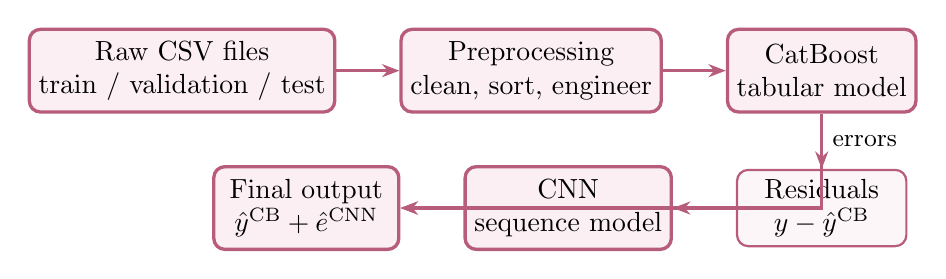
\begin{tikzpicture}[
    node distance=7mm and 8mm,
    box/.style={rounded corners, draw=softpinkdark, very thick, fill=softpink!45, align=center, minimum width=2.35cm, minimum height=1.05cm},
    smallbox/.style={rounded corners, draw=softpinkdark, thick, fill=softpink!25, align=center, minimum width=2.15cm, minimum height=0.9cm},
    arrow/.style={-{Stealth[length=2.2mm]}, very thick, draw=softpinkdark}
  ]
    \node[box] (raw) {Raw CSV files\\train / validation / test};
    \node[box, right=of raw] (prep) {Preprocessing\\clean, sort, engineer};
    \node[box, right=of prep] (cb) {CatBoost\\tabular model};
    \node[smallbox, below=of cb] (res) {Residuals\\$y-\hat y^{\mathrm{CB}}$};
    \node[box, left=of res] (cnn) {CNN\\sequence model};
    \node[box, left=of cnn] (final) {Final output\\$\hat y^{\mathrm{CB}}+\hat e^{\mathrm{CNN}}$};

    \draw[arrow] (raw) -- (prep);
    \draw[arrow] (prep) -- (cb);
    \draw[arrow] (cb) -- node[right, font=\small] {errors} (res);
    \draw[arrow] (res) -- (cnn);
    \draw[arrow] (cnn) -- (final);
    \draw[arrow] (cb) |- (final);
  \end{tikzpicture}

  \vspace{0.4em}
  \begin{itemize}
    \item The top path learns the main tabular pattern.
    \item The bottom path learns the leftover time pattern.
  \end{itemize}
\end{frame}

\begin{frame}{What This Project Does}
  \begin{itemize}
    \item The goal is to estimate $y_{j,t}$ for each company-month pair $(j,t)$.
    \item The data form a monthly panel $\{(j,t,r_{j,t})\}$.
    \item The model is split into two parts:
    \begin{itemize}
      \item CatBoost learns $f_{\mathrm{CB}}(x_{j,t})$.
      \item CNN learns the residual $e_{j,t} = y_{j,t} - \hat y^{\mathrm{CB}}_{j,t}$.
    \end{itemize}
    \item The pipeline preserves chronology and prevents leakage: $\tau \le t$ only.
  \end{itemize}
\end{frame}

\begin{frame}{Big Picture Flow}
  \begin{enumerate}
    \item Load $\D_{\mathrm{train}}$, $\D_{\mathrm{val}}$, and $\D_{\mathrm{test}}$.
    \item Build $x_{j,t}=\phi(\{r_{j,\tau}:\tau\le t\})$.
    \item Fit $\hat f_{\mathrm{CB}}$ on tabular features.
    \item Compute $e_{j,t}=y_{j,t}-\hat y^{\mathrm{CB}}_{j,t}$.
    \item Fit $\hat f_{\mathrm{CNN}}$ on sequence tensors $\seq_{j,t}$.
    \item Predict $\hat y_{j,t}=\hat y^{\mathrm{CB}}_{j,t}+\hat e^{\mathrm{CNN}}_{j,t}$.
    \item Store metrics, predictions, and HTML logs.
  \end{enumerate}
\end{frame}

\begin{frame}{Why Use Two Models?}
  \begin{itemize}
    \item CatBoost models $x_{j,t} \in \mathbb{R}^d$.
    \item It handles numerical and categorical structure well.
    \item Some signal is temporal and lives in the residuals.
    \item CNN models short windows $\seq_{j,t} \in \mathbb{R}^{d \times L}$.
    \item The final prediction is the sum of both parts:
    \[
      \haty_{j,t} = \haty^{\mathrm{CB}}_{j,t} + \haty^{\mathrm{CNN}}_{j,t}.
    \]
  \end{itemize}
\end{frame}

\begin{frame}{Simple View of the Math}
  Let:
  \begin{itemize}
    \item $y_{j,t}$ be the true return for company $j$ at month $t$,
    \item $x_{j,t}$ be the feature vector for that row,
    \item $\seq_{j,t}$ be the short sequence used by the CNN.
  \end{itemize}

  The model works like this:
  \[
    y_{j,t} \approx f_{\mathrm{CB}}(x_{j,t}) + f_{\mathrm{CNN}}(\seq_{j,t}).
  \]

  In plain language:
  \begin{itemize}
    \item CatBoost explains the obvious part.
    \item CNN explains the leftover part.
  \end{itemize}
\end{frame}

\begin{frame}{How The Data Is Processed}
  \begin{itemize}
    \item The raw row for company $j$ at month $t$ is called $r_{j,t}$.
    \item Preprocessing creates a cleaned feature row $x_{j,t}$.
    \item The cleaned row depends only on current and past months:
    \[
      x_{j,t} = \phi\big(\{r_{j,\tau} : \tau \le t\}\big).
    \]
    \item This keeps the pipeline leakage-safe and causal.
    \item Lags and rolling features use $t-1,t-3,t-6$ style history.
  \end{itemize}
\end{frame}

\begin{frame}{Feature Construction Math}
  \begin{block}{Lag features}
    For lag $\ell \in \{1,3,6\}$, the lag feature is the earlier target value:
    \[
      \mathrm{lag\_ret}_\ell(j,t) = y_{j,t-\ell}.
    \]
  \end{block}

  \begin{block}{Rolling features}
    A rolling mean over window $w$ is computed from past values only:
    \[
      \mathrm{rolling\_mean}_w(j,t) = \frac{1}{|I_{j,t}^{(w)}|}\sum_{\tau \in I_{j,t}^{(w)}} y_{j,\tau}.
    \]
    The same idea is used for rolling standard deviation.
  \end{block}
\end{frame}

\begin{frame}{CatBoost in Plain Language}
  \begin{itemize}
    \item CatBoost is a boosting model made of many small decision trees.
    \item Each new tree tries to fix the mistakes of the previous trees.
    \item After many steps, the model becomes a strong predictor.
    \item It works well when features are a mix of numeric values and categories.
  \end{itemize}

  A simple training objective is:
  \[
    \loss_{\mathrm{CB}} = \frac{1}{n} \sum_{i=1}^{n} (y_i - \haty_i)^2.
  \]
\end{frame}

\begin{frame}{How Boosting Works}
  \begin{itemize}
    \item Start with a simple guess, usually the average target.
    \item Measure the error made by that guess.
    \item Train a small tree to predict the error.
    \item Add the tree to the current model.
    \item Repeat many times until the error is low enough.
  \end{itemize}

  In symbol form:
  \[
    F_M(x) = F_0(x) + \sum_{m=1}^{M} \eta_m h_m(x),
  \]
  where each $h_m$ is a small tree and $\eta_m$ is the step size.
\end{frame}

\begin{frame}{Preprocessing Pipeline}
  \begin{itemize}
    \item Load $\D_{\mathrm{train}},\D_{\mathrm{val}},\D_{\mathrm{test}}$.
    \item Concatenate temporarily: $\D = \D_{\mathrm{train}} \cup \D_{
    \mathrm{val}} \cup \D_{\mathrm{test}}$.
    \item Sort by $(\mathrm{co\_code}, \mathrm{Month})$.
    \item Collapse duplicate keys $(j,t)$.
    \item Coerce $\mathrm{Month}$, $\mathrm{co\_code}$, and $y_{j,t}$.
    \item Build $\mathrm{lag\_ret}_\ell$, $\mathrm{rolling\_mean}_w$, and missing flags.
    \item Recover the original split sets.
  \end{itemize}
\end{frame}

\begin{frame}{Implementation Details Used In Code}
  \begin{itemize}
    \item Duplicate company--month rows are collapsed by keeping the last observation.
    \item Missing categorical values are filled with \texttt{\_\_MISSING\_\_}.
    \item Lag steps are set to 1, 3, and 6 months.
    \item Rolling windows are set to 3 and 6 months.
    \item CNN sequences use a window length of 6.
    \item CatBoost predictions are stored as \texttt{cb\_pred}.
    \item Residual targets are stored as \texttt{base\_residual} and \texttt{residual\_target}.
  \end{itemize}
\end{frame}

\begin{frame}{Why Preprocessing Matters}
  \begin{itemize}
    \item Financial panel data are time ordered.
    \item We must not use future months when building features for past rows.
    \item Lag features use only earlier months.
    \item Rolling features also look only backward in time.
    \item Missing-value flags help the model learn when data are absent.
  \end{itemize}
\end{frame}

\begin{frame}{CatBoost Training in This Project}
  \begin{itemize}
    \item Train CatBoost only on $\D_{\mathrm{train}}$.
    \item Use $\D_{\mathrm{val}}$ for model checking and early stopping.
    \item Pass categorical features directly into the Pool.
    \item Predict on $\D_{\mathrm{val}}$ and $\D_{\mathrm{test}}$.
    \item Compute residuals:
    \[
      e_{j,t} = y_{j,t} - \haty^{\mathrm{CB}}_{j,t}.
    \]
  \end{itemize}
\end{frame}

\begin{frame}{CNN Training in This Project}
  \begin{itemize}
    \item CNN uses a window $\seq_{j,t} \in \mathbb{R}^{d \times L}$.
    \item Each window is standardized with training statistics $(\mu,\sigma)$.
    \item The CNN estimates $\hat e^{\mathrm{CNN}}_{j,t}$, not $y_{j,t}$ directly.
    \item The loss is mean squared error on residuals:
    \[
      \loss_{\mathrm{CNN}} = \frac{1}{m} \sum_{i=1}^{m} (e_i - \hat e_i)^2.
    \]
  \end{itemize}
\end{frame}

\begin{frame}{CNN Block Diagram}
  \centering
  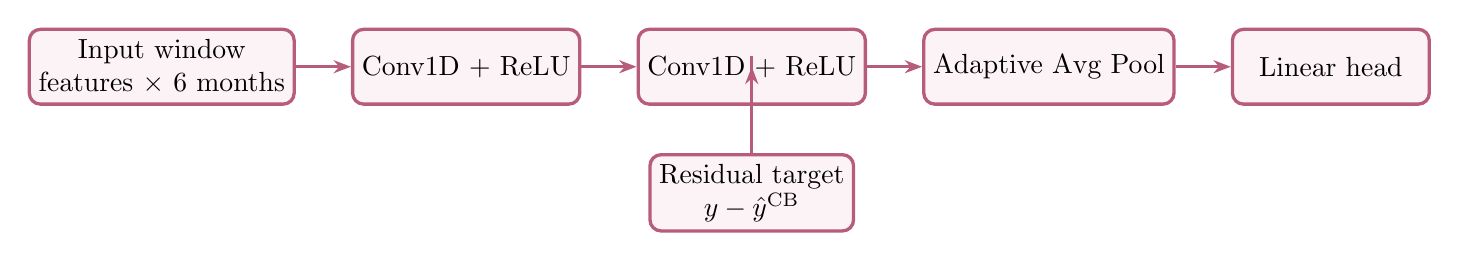
\begin{tikzpicture}[
    node distance=6mm and 7mm,
    layer/.style={rounded corners, draw=softpinkdark, very thick, fill=softpink!35, align=center, minimum width=2.5cm, minimum height=0.95cm},
    arrow/.style={-{Stealth[length=2.2mm]}, very thick, draw=softpinkdark}
  ]
    \node[layer] (input) {Input window\\features $\times$ 6 months};
    \node[layer, right=of input] (conv1) {Conv1D + ReLU};
    \node[layer, right=of conv1] (conv2) {Conv1D + ReLU};
    \node[layer, right=of conv2] (pool) {Adaptive Avg Pool};
    \node[layer, right=of pool] (head) {Linear head};
    \node[layer, below=of conv2] (resid) {Residual target\\$y-\hat y^{\mathrm{CB}}$};

    \draw[arrow] (input) -- (conv1);
    \draw[arrow] (conv1) -- (conv2);
    \draw[arrow] (conv2) -- (pool);
    \draw[arrow] (pool) -- (head);
    \draw[arrow] (resid) |- (conv2);
  \end{tikzpicture}

  \vspace{0.4em}
  \begin{itemize}
    \item The CNN sees a window of past rows, not a single row.
    \item The output is one correction value for the target return.
  \end{itemize}
\end{frame}

\begin{frame}{How the CNN Sees the Data}
  \begin{itemize}
    \item Input shape is roughly: features \(\times\) time window.
    \item Convolution layers scan across the time axis.
    \item This helps the model detect local patterns such as short momentum or reversal effects.
    \item After convolution, the model uses pooling and a linear output layer.
  \end{itemize}
\end{frame}

\begin{frame}{Inference and Logging}
  \begin{itemize}
    \item At inference time, append new rows to the historical panel.
    \item Rebuild features with the same map $\phi$.
    \item Predict $\hat y^{\mathrm{CB}}_{j,t}$ first.
    \item Build a valid window $\seq_{j,t}$ if $|H_{j,t}| \ge L$.
    \item Add the CNN correction and write $\hat y_{j,t}$.
    \item Save outputs, metrics, and HTML summaries.
  \end{itemize}
\end{frame}

\begin{frame}{What Gets Logged}
  \begin{itemize}
    \item Final predictions $\hat y_{j,t}$ for each row.
    \item Base predictions $\hat y^{\mathrm{CB}}_{j,t}$ and corrections $\hat e^{\mathrm{CNN}}_{j,t}$.
    \item Metrics such as RMSE, MAE, $R^2$, and directional accuracy.
    \item Learning curves for CatBoost and CNN.
    \item Error distributions and monthly summaries.
  \end{itemize}
\end{frame}

\begin{frame}{Takeaway}
  \begin{itemize}
    \item CatBoost handles the main tabular structure.
    \item CNN handles the leftover time pattern in the residuals.
    \item Preprocessing protects against leakage.
    \item Inference repeats the same logic used during training.
    \item Logging makes the model easier to inspect and compare.
  \end{itemize}
\end{frame}

\end{document}
